% Moved verbatim from Paper A (new/sections/results.tex lines 226-254 and table row 279, commit f96523f) on 2026-10-29. Raw material for Paper B; rewrite, do not reuse.
\begin{figure}[t]
  \centering
  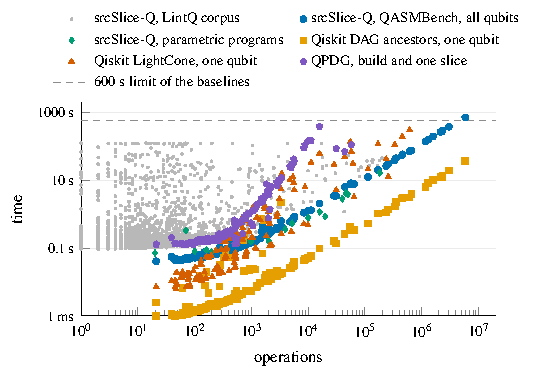
\includegraphics[width=\columnwidth]{figures/fig_scale.pdf}
  \caption{Time of \tool{} against the operations of a trace, for RQ4. Grey points are the programs of LintQ's corpus,
  with every stage. The QASMBench points slice every qubit in one pass, reading included, and the baselines slice one
  qubit of the same circuits, loading included. Runs beyond the 600~s limit are left out.}
  \label{fig:scale}
\end{figure}

\tool{} scales to the programs developers write and to circuits of millions of operations, as Fig.~\ref{fig:scale}
shows. On LintQ's corpus it slices the \numScaleSOneSliced{} programs that build a circuit, every qubit up to 64 of
them, in \numScaleSOneMedianMs{}~ms per program in the median and within \numScaleSOneNinetyNine{}~s for 99\% of them,
and \numScaleSOneTimeouts{} programs reach the limit of 120~s. srcML and srcSlice take most of the median,
\numScaleSOneSrcmlMs{} and \numScaleSOneSrcsliceMs{}~ms, and the slices themselves \numScaleSOneSliceMs{}~ms. A qubit's
slice holds \numScaleReadMedianPct{} of a program's code lines in the median. On the \numScaleQbRead{} QASMBench circuits
in valid OpenQASM~2, of up to \numScaleQbMaxOps{} operations and \numScaleQbMaxQubits{} qubits, the one-pass slice of
every qubit takes at most \numScaleQbAllS{}~s, on the largest circuit, after \numScaleQbReadS{}~s of reading. Qiskit's
DAG slices one of its \numScaleQbMaxOpsQubits{} qubits in \numScaleQbDagOneS{}~s after \numScaleQbDagLoadS{}~s of loading,
about \numScaleQbDagAllMin{} minutes for all of them. Qubit for qubit the two are close, \tool{}'s single slice taking
\numScaleOneRatio{} times Qiskit's in the median and \numScaleOneRatioBig{} times on circuits of 100{,}000 operations or
more, so \tool{}'s advantage is the single pass over every qubit. The QPDG reimplementation builds its graph within the
limit for circuits of up to \numScaleQpdgMaxOps{} operations, in \numScaleQpdgMaxS{}~s, where \tool{} reads and slices
the circuit in \numScaleQpdgSqS{}~s, and the \numScaleQpdgOver{} larger circuits are beyond it. Qiskit's \texttt{LightCone}
pass slices one qubit of the circuit of \numScaleLcMaxOps{} operations in \numScaleLcMaxS{}~s, where \tool{} slices all
\numScaleLcQubits{} of its qubits in \numScaleLcSqS{}~s, and exceeds the limit on \numScaleLcOver{} circuits. On the
parametric programs the source stays at about a dozen lines while the trace grows. The QFT on 600 qubits unrolls
\numScaleQftOps{} operations from \numScaleQftLines{} code lines in \numScaleQftS{}~s, where running the program with
Qiskit and slicing one qubit takes \numScaleQftRunS{}~s, the speed a static slicer gives up so that it never executes
the program.
% Table VIII row:
    Largest circuit within the limit & \win\numScaleQbMaxOps{} & \numScaleQpdgMaxOps{} & RQ4 \\
